\documentclass{standalone}
\usepackage[centertags]{amsmath}
\usepackage{latexsym}
\usepackage{amsfonts}
\usepackage{amssymb}
\usepackage{amsthm}
\usepackage{newlfont}
\usepackage{enumerate}
\usepackage{makeidx}
\usepackage{tikz}
\usetikzlibrary{backgrounds,intersections}
\begin{document}
        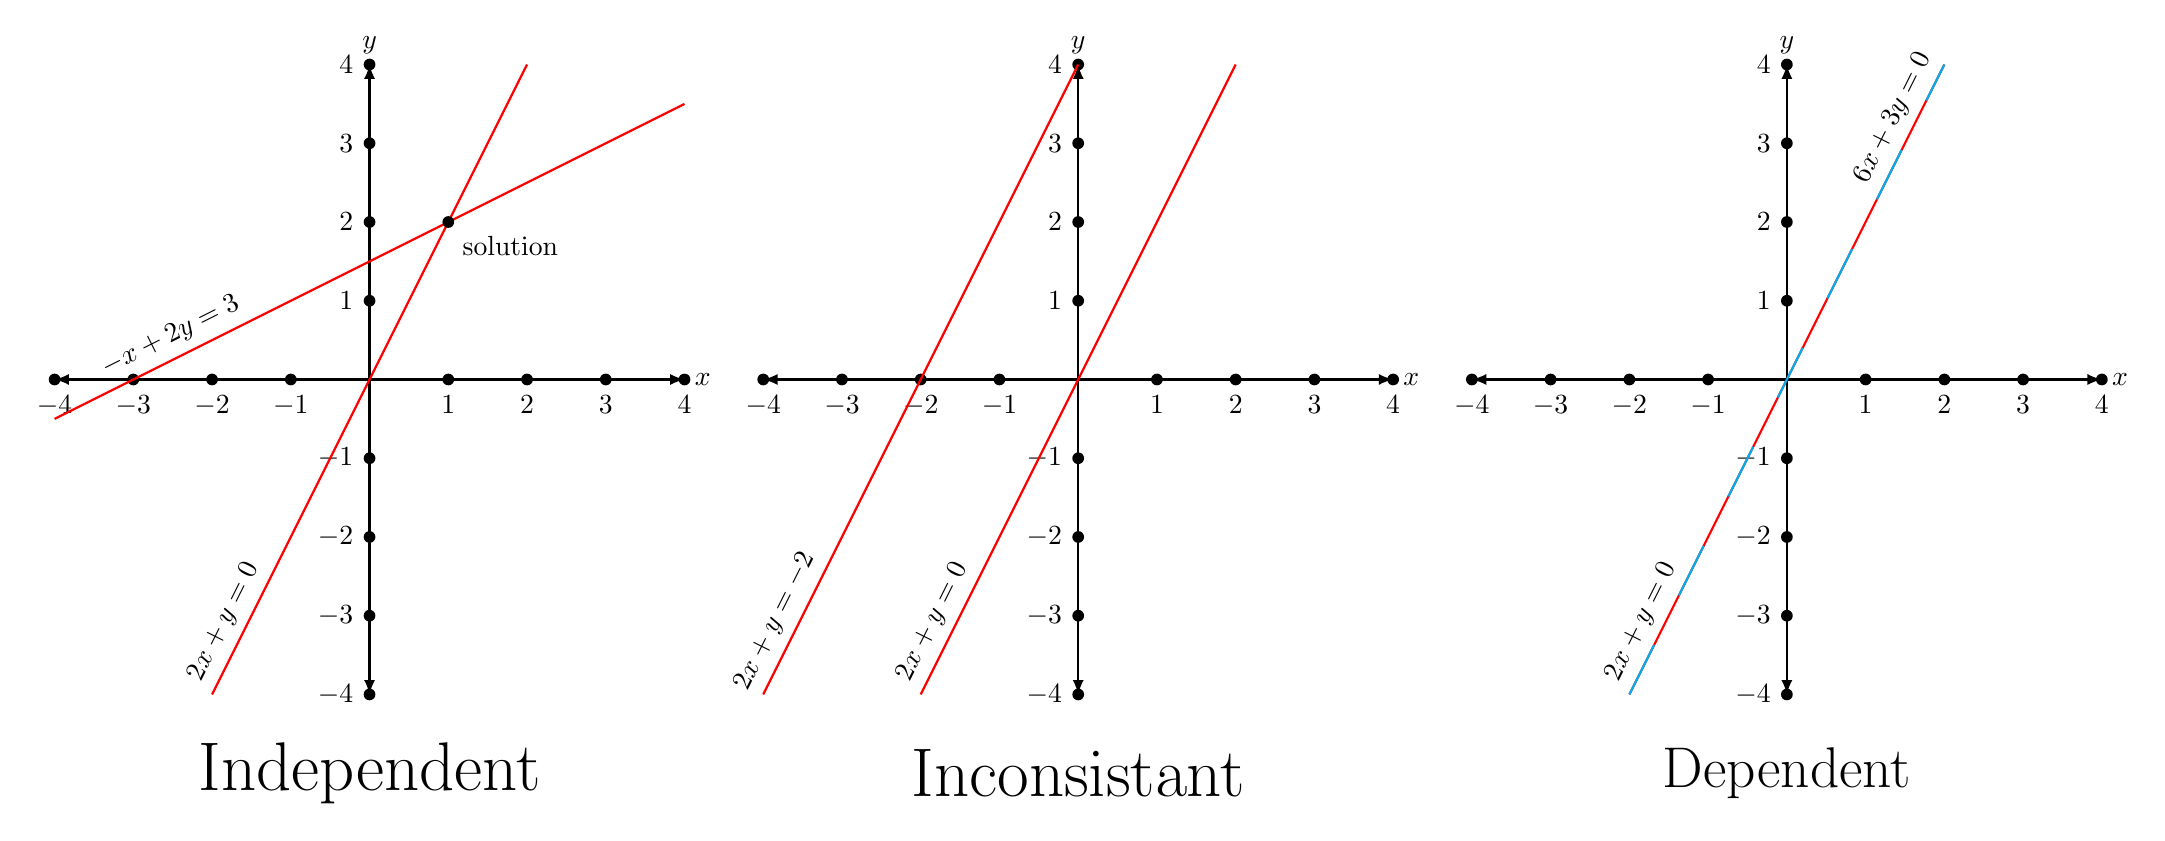
\begin{tikzpicture}
	\draw[thick,latex-latex] (-4,0) -- (4,0)node[right]{$x$};
        \draw[thick,latex-latex] (0,-4) -- (0,4)node[above]{$y$};
        \foreach \x in {-4,-3,-2,-1,1,2,3,4}{
            \node[fill,circle,inner sep=1.5pt,label=below:$\x$] at (\x,0) {};
            \node[fill,circle,inner sep=1.5pt,label=left:$\x$] at (0,\x) {};
        }
        \draw[red,thick] (-4,-0.5) -- (4,3.5)
        node[pos=0.2,black,above,sloped] {$-x+2y=3$};
        \draw[red,thick] (-2,-4) -- (2,4)
        node[pos=0.1,black,above,sloped] {$2x+y=0$};
	\node[fill,circle,inner sep=1.5pt,label=below right:solution] at (1,2) {};
	\node at(0, -5){\Huge Independent};
	

	\draw[thick,latex-latex] (5,0) -- (13,0)node[right]{$x$};
        \draw[thick,latex-latex] (9,-4) -- (9,4)node[above]{$y$};
        \foreach \x in {-4,-3,-2,-1,1,2,3,4}{
		\node[fill,circle,inner sep=1.5pt,label=below:$\x$] at ({\x+9},0) {};
		\node[fill,circle,inner sep=1.5pt,label=left:$\x$] at (9,\x) {};
        }

	\draw[red,thick] ({-2+7},-4) -- ({2+7},4)
        node[pos=0.1,black,above,sloped] {$2x+y=-2$};
	\draw[red,thick] ({-2+9},-4) -- ({2+9},4)
        node[pos=0.1,black,above,sloped] {$2x+y=0$};
	\node at(9, -5){\Huge Inconsistant};


	\draw[thick,latex-latex] (14,0) -- (22,0)node[right]{$x$};
         \foreach \x in {-4,-3,-2,-1,1,2,3,4}{
		\node[fill,circle,inner sep=1.5pt,label=below:$\x$] at ({\x+18},0) {};
		\node[fill,circle,inner sep=1.5pt,label=left:$\x$] at (18,\x) {};
        }
       \draw[thick,latex-latex] (18,-4) -- (18,4)node[above]{$y$};
	\draw[red,thick] ({-2+18},-4) -- ({2+18},4)
        node[pos=0.1,black,above,sloped] {$2x+y=0$}
        node[pos=0.9,black,above,sloped] {$6x+3y=0$};
	\draw[cyan,thick,dash pattern=on 2em off 2em] ({-2+18},-4) -- ({2+18},4);
	\node at(18, -5){\huge Dependent};
        \end{tikzpicture}
\end{document}
